\documentclass[10pt, a4paper]{article}
\usepackage[a4paper, left=1.4cm, right=1.4cm, top=0.9cm, bottom=0.9cm]{geometry}
\usepackage{fontspec}
\setmainfont{Helvetica Neue}
\usepackage{tikz}
\usepackage{eso-pic}
\usepackage{lastpage}
\usepackage{refcount}
\usepackage{xcolor}
\usepackage{enumitem}
\usepackage[nolinks]{qrcode}
\pagestyle{empty}
\setlength{\parindent}{0pt}
\setlength{\parskip}{2pt}
\newcommand{\bub}[1]{\begin{tikzpicture}[baseline=-0.6ex]\draw[line width=1.2pt](0,0) circle (8pt);\node[font=\fontsize{7.2}{7.2}\selectfont\bfseries] at (0,0){#1};\end{tikzpicture}\hspace{4pt}}
\newcommand{\questionblock}[2]{\vspace{4pt}\textbf{Q#1.} #2\par}
\newcommand{\answerline}[2]{\textbf{Answer Q#1}\quad #2\par}
\newcommand{\bqpagepayload}{bubblequiz|course=BES2041|version=4|questions=1,2,3,4,5,6|page=\the\value{page}|pages=\getpagerefnumber{LastPage}}
\newcommand{\bqpageqr}{\expanded{\noexpand\qrcode[height=1.3cm]{\bqpagepayload}}}
\AddToShipoutPictureBG{%
\begin{tikzpicture}[remember picture, overlay]
  \fill[black] ([xshift= 3mm, yshift= -3mm]current page.north west) rectangle ++( 5mm, -5mm);
  \fill[black] ([xshift=-8mm, yshift= -3mm]current page.north east) rectangle ++( 5mm, -5mm);
  \fill[black] ([xshift= 3mm, yshift=  3mm]current page.south west) rectangle ++( 5mm,  5mm);
  \fill[black] ([xshift=-8mm, yshift=  3mm]current page.south east) rectangle ++( 5mm,  5mm);
  \node[anchor=south west, inner sep=0pt, font=\footnotesize] at ([xshift=11mm, yshift=4mm]current page.south west) {\ifnum\value{page}>1 \textbf{Name}~\underline{\hspace{55mm}}\quad\fi Page \thepage\ of \pageref{LastPage}};
  \node[anchor=south east, inner sep=0pt] at ([xshift=-12mm, yshift=3mm]current page.south east) {\bqpageqr};
\end{tikzpicture}}
\begin{document}
\begin{minipage}[t]{0.70\linewidth}
{\LARGE\bfseries BES2041 Lecture Quiz Test}\\[1pt]
{\normalsize Multiple Choice Quiz}
\end{minipage}\hfill
\begin{minipage}[t]{0.28\linewidth}\raggedleft
\colorbox{black}{\textcolor{white}{\large\bfseries\quad Version 4\quad}}\\[2pt]
{\footnotesize 16 September 2026}
\end{minipage}\\[2pt]
\rule{\linewidth}{1.2pt}
\begin{minipage}[t]{0.40\linewidth}
\vspace{2pt}
\textbf{Name}\quad\underline{\hspace{0.74\linewidth}}
\end{minipage}\hfill
\begin{minipage}[t]{0.56\linewidth}
\vspace{2pt}
\textbf{Fill zID digit bubbles:}\\[-2pt]
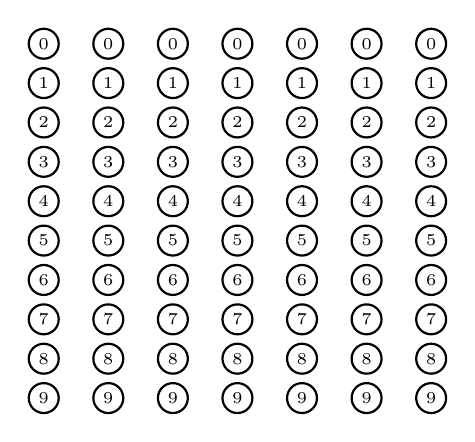
\begin{tikzpicture}[x=0.82cm, y=-0.50cm]\foreach \col in {0,...,6}{\foreach \d in {0,...,9}{\draw[line width=0.8pt](\col, \d) circle (0.19cm);\node[font=\fontsize{6.4}{6.4}\selectfont] at (\col, \d) {\d};}}\end{tikzpicture}
\end{minipage}
\vspace{3pt}\rule{\linewidth}{1.2pt}
\begin{samepage}
\questionblock{1}{In fieldwork you often tape the circumference of a tree at breast height but need diameter (DBH) to use a height–DBH model. What is the correct conversion from measured circumference C to diameter d?}
\begin{enumerate}[label=\alph*., leftmargin=1.4em, itemsep=1pt, topsep=2pt]
  \item d = 2C / π
  \item d = πC
  \item d = √(C/π)
  \item d = C² / π
  \item d = C / π
\end{enumerate}
\answerline{1}{\bub{A}\bub{B}\bub{C}\bub{D}\bub{E}}
\vspace{5pt}
\end{samepage}
\begin{samepage}
\questionblock{2}{You are comparing two models that predict a vegetation variable Y from a sensor index X. Your priority is to minimise absolute prediction error in interpretable units of Y. Which metric should guide your choice?}
\begin{enumerate}[label=\alph*., leftmargin=1.4em, itemsep=1pt, topsep=2pt]
  \item R²
  \item Correlation coefficient r
  \item p-value of the slope
  \item Root Mean Squared Error (RMSE)
  \item Adjusted R²
\end{enumerate}
\answerline{2}{\bub{A}\bub{B}\bub{C}\bub{D}\bub{E}}
\vspace{5pt}
\end{samepage}
\begin{samepage}
\questionblock{3}{You can easily measure DBH but not height in a forest survey. Which workflow best matches the lecture’s definition of a model and the purpose of prediction?}
\begin{enumerate}[label=\alph*., leftmargin=1.4em, itemsep=1pt, topsep=2pt]
  \item Use Pythagoras with GPS coordinates to compute tree height from planimetric distances.
  \item Measure a few heights, take the mean, and assign it to all trees.
  \item Map crowns in an equal-area projection and use crown area as height proxies.
  \item Assume a fixed height:diameter ratio from a paper and multiply all DBHs by that constant.
  \item Fit a statistical model of height from DBH using a training set, then use it to predict heights for the remaining trees.
\end{enumerate}
\answerline{3}{\bub{A}\bub{B}\bub{C}\bub{D}\bub{E}}
\vspace{5pt}
\end{samepage}
\begin{samepage}
\questionblock{4}{Why did the lecture emphasize using simple formulae carefully before moving into software tools?}
\begin{enumerate}[label=\alph*., leftmargin=1.4em, itemsep=1pt, topsep=2pt]
  \item Quantitative interpretation still depends on understanding what measurements and formulae represent.
  \item Environmental science avoids mathematical calculations once data are collected.
  \item Formulae are only relevant for drawing figures, not analysis.
  \item Coding removes the need to think about units or measurement.
  \item Software can only run if every formula is typed from memory.
\end{enumerate}
\answerline{4}{\bub{A}\bub{B}\bub{C}\bub{D}\bub{E}}
\vspace{5pt}
\end{samepage}
\begin{samepage}
\questionblock{5}{In the lecture, what was the purpose of discussing RStudio setup before the labs?}
\begin{enumerate}[label=\alph*., leftmargin=1.4em, itemsep=1pt, topsep=2pt]
  \item To replace all later lectures with self-guided programming tasks.
  \item To assess students before they had seen the course material.
  \item To demonstrate that coding is separate from environmental science.
  \item To discourage students from using local computers.
  \item To make sure students could use the required computing environment for practical work.
\end{enumerate}
\answerline{5}{\bub{A}\bub{B}\bub{C}\bub{D}\bub{E}}
\vspace{5pt}
\end{samepage}
\begin{samepage}
\questionblock{6}{Which statement best describes the role of a cloud workaround such as Google Colab in the lecture?}
\begin{enumerate}[label=\alph*., leftmargin=1.4em, itemsep=1pt, topsep=2pt]
  \item It is a backup option for students who cannot run the local software environment.
  \item It automatically calculates all answers without coding.
  \item It is required before students can learn RStudio.
  \item It is used only for watching lecture videos.
  \item It is the default tool for all students regardless of their computer setup.
\end{enumerate}
\answerline{6}{\bub{A}\bub{B}\bub{C}\bub{D}\bub{E}}
\vspace{5pt}
\end{samepage}
\end{document}
